%%%%%%%%%%%%%%%%%%%%%%%%%%%%%%%%%%%%%%%%%%%%%%%%%%%%%%%%%%%%%%%%%%%%%%%%%%%%%%%%%%%%%%%%%%%%%%%%%%%
% Chapter 5 -> Results
% Author: Mingbo Cheng
%%%%%%%%%%%%%%%%%%%%%%%%%%%%%%%%%%%%%%%%%%%%%%%%%%%%%%%%%%%%%%%%%%%%%%%%%%%%%%%%%%%%%%%%%%%%%%%%%%%
\chapter{Results}
\label{chapter:results}

\graphicspath{{chapter5/figs}}

\section{Technique Validatation}
\subsection{Data}
\subsection{Execution of multi-modal integration}
\subsection{Evaluation of multi-modal integration}


\begin{figure}[!ht]
	\centering
	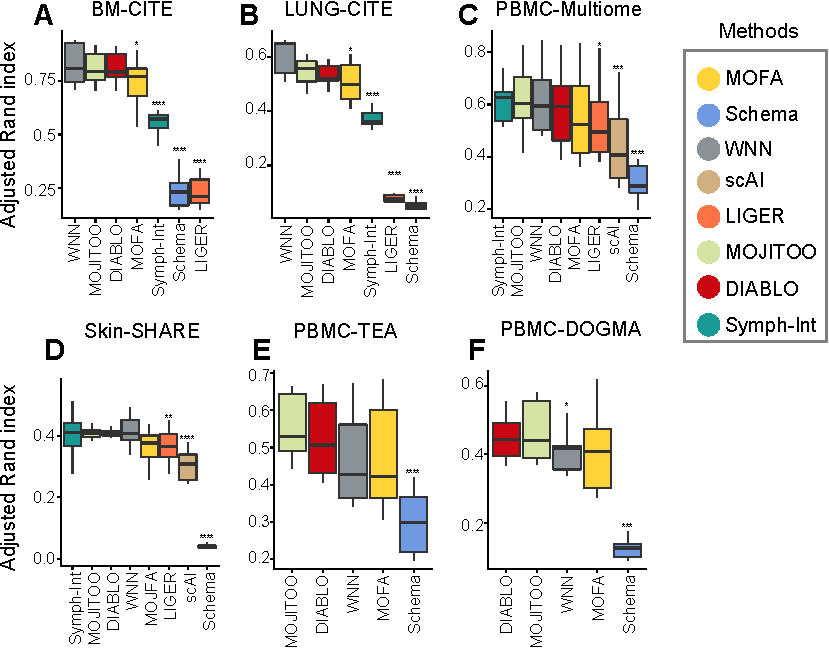
\includegraphics[width=0.95\textwidth]{ari/fig}
	\vspace{0.1cm}
	\caption[Evaluation of clustering accuracy for multi-modal integration methods.]{Evaluation of clustering accuracy for multi-modal integration methods.}
	\label{fig:ari}
\end{figure}


\begin{figure}[!ht]
	\centering
	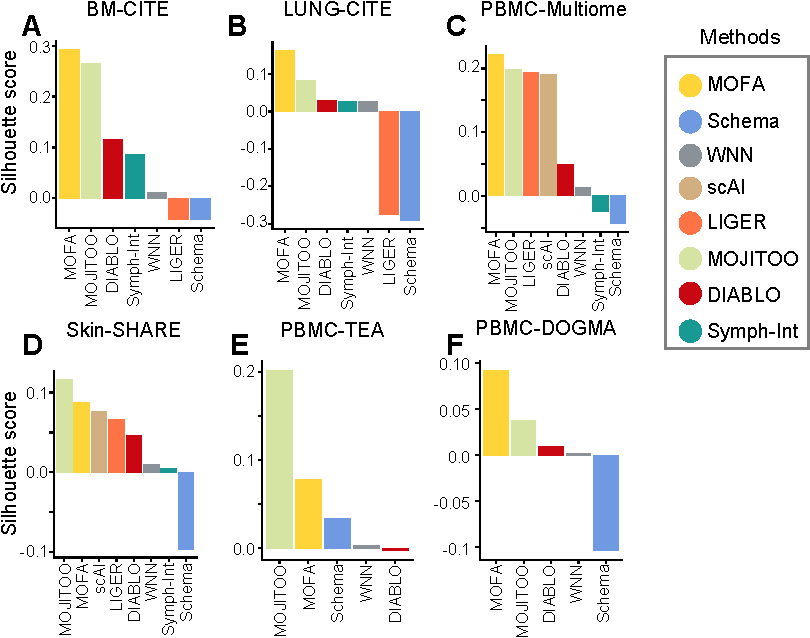
\includegraphics[width=0.95\textwidth]{silouette/fig}
	\vspace{0.1cm}
	\caption[Evaluation of distance accuracy for multi-modal integration methods.]{
        Evaluation of distance accuracy for multi-modal integration methods.}
	\label{fig:silouette}
\end{figure}


\begin{figure}[!ht]
	\centering
	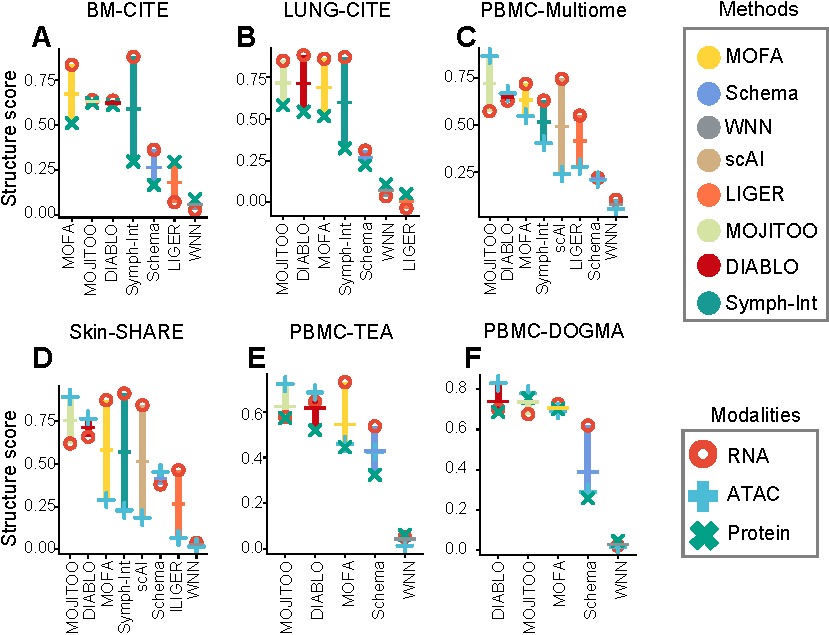
\includegraphics[width=0.95\textwidth]{structure/fig}
	\vspace{0.1cm}
	\caption[Evaluation of space preservation for multi-modal integration methods.]{Evaluation of space preservation for multi-modal integration methods.}
	\label{fig:structure}
\end{figure}

\begin{figure}[!ht]
	\centering
	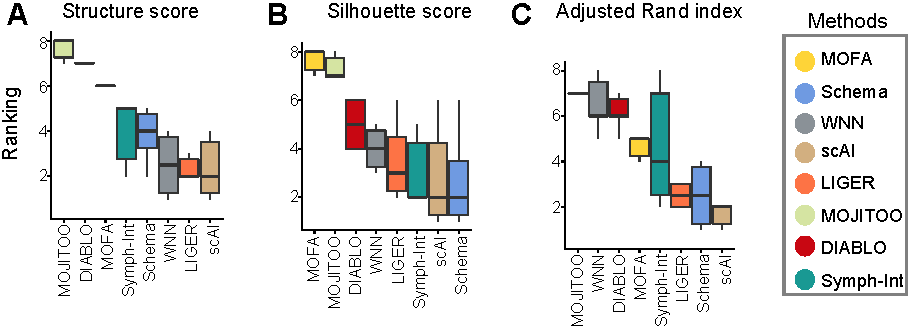
\includegraphics[width=0.95\textwidth]{ranking/fig}
	\vspace{0.1cm}
	\caption[Evaluation of ranking for multi-modal integration methods.]{Evaluation of ranking for multi-modal integration methods.}
	\label{fig:ranking}
\end{figure}


\begin{figure}[!ht]
	\centering
	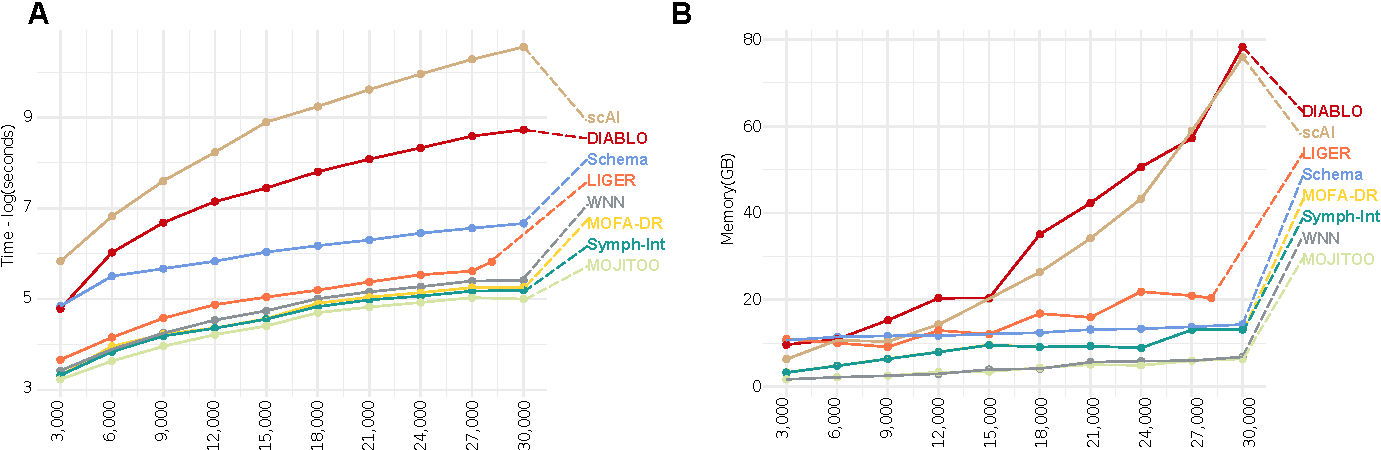
\includegraphics[width=0.95\textwidth]{time_memory/fig}
	\vspace{0.1cm}
	\caption[Evaluation of time and memory consumption for multi-modal integration methods.]{Evaluation of time and memory consumption for multi-modal integration methods.}
	\label{fig:time_memory}
\end{figure}

\begin{figure}[!ht]
	\centering
	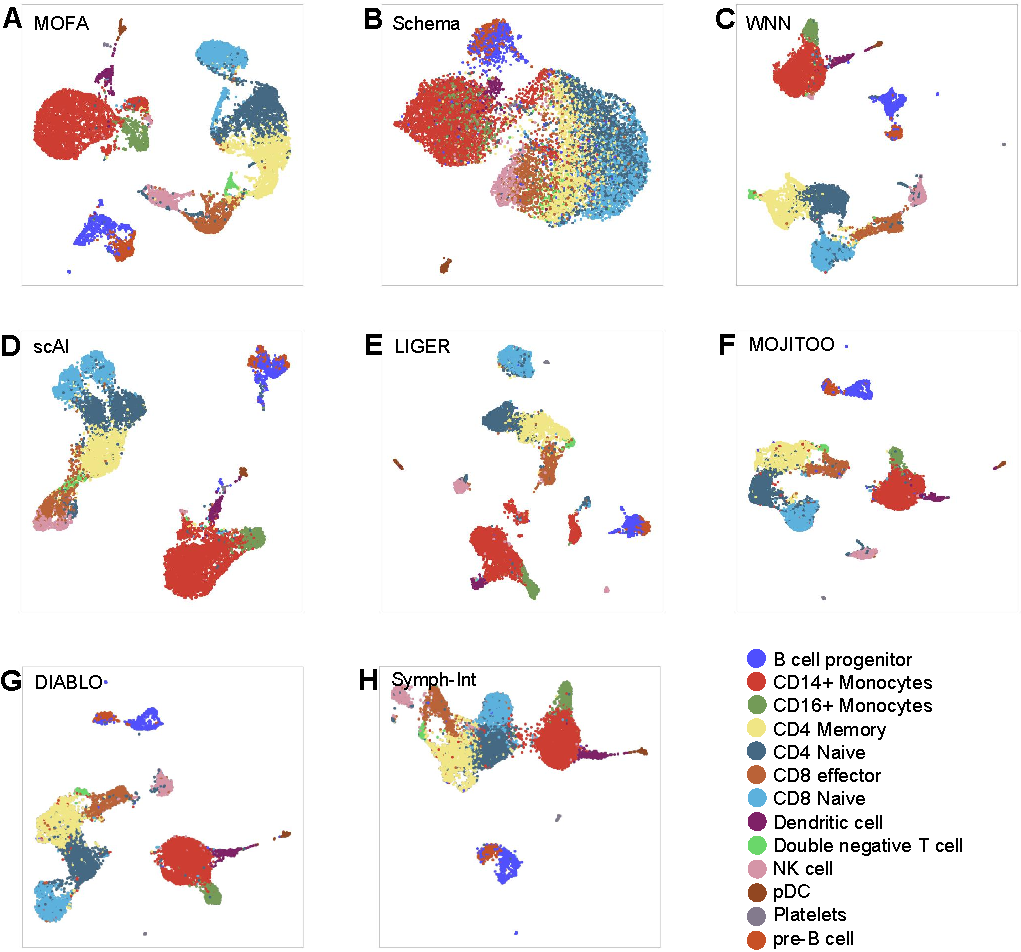
\includegraphics[width=0.95\textwidth]{pbmc_multiome_umap/fig}
	\vspace{0.1cm}
	\caption[UMAP of multiome PBMC comparison for different multi-modal integration methods.]{UMAP of multiome PBMC comparison for different multi-modal integration methods.}
	\label{fig:pbmc_multiome_umap}
\end{figure}


\begin{figure}[!ht]
	\centering
	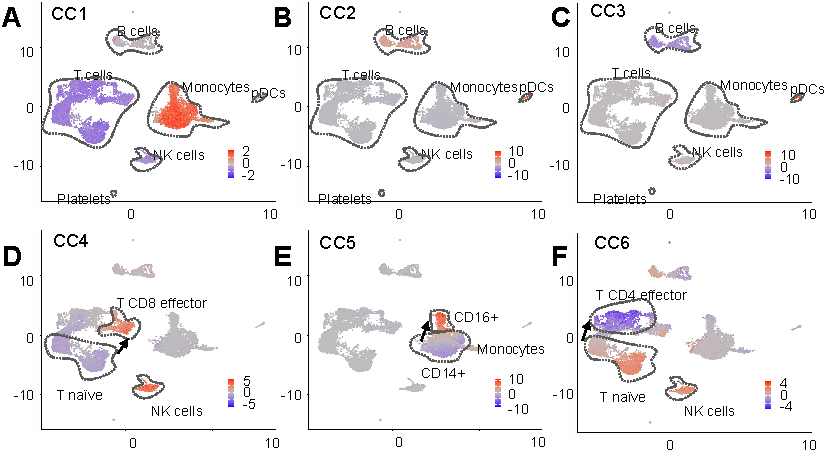
\includegraphics[width=0.95\textwidth]{CC_UMAP/fig}
	\vspace{0.1cm}
	\caption[CCs in the UMAP.]{CCs in the UMAP.}
	\label{fig:CC_UMAP}
\end{figure}





\begin{figure}[!ht]
	\centering
	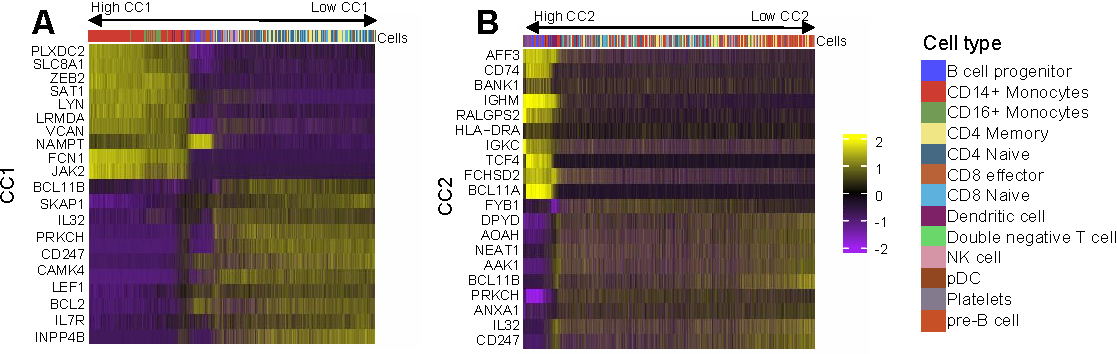
\includegraphics[width=0.95\textwidth]{CC_Genes/fig}
	\vspace{0.1cm}
	\caption[UMAP of multiome PBMC comparison for different multi-modal integration methods.]{UMAP of multiome PBMC comparison for different multi-modal integration methods.}
	\label{fig:CC_Genes}
\end{figure}



\begin{figure}[!ht]
	\centering
	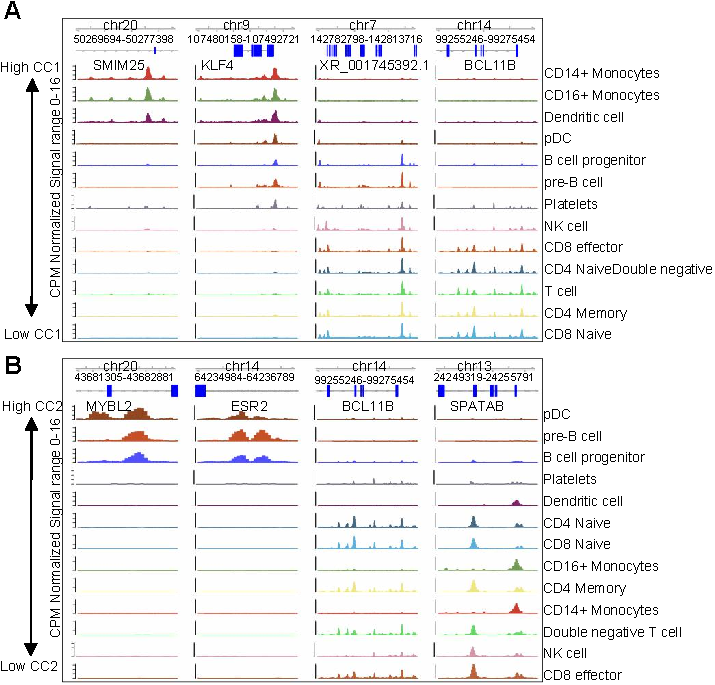
\includegraphics[width=0.95\textwidth]{CC_Peaks/fig}
	\vspace{0.1cm}
	\caption[UMAP of multiome PBMC comparison for different multi-modal integration methods.]{UMAP of multiome PBMC comparison for different multi-modal integration methods.}
	\label{fig:CC_Peaks}
\end{figure}





\subsection{Execution of trajectory inference}


\subsection{Evaluation of trajectory inference}

\section{Biological Validatation}
\subsection{Apply integration \& trajectory inference to kidney organoid data}
\subsection{Characterize the cell fate xxxx}

\section{Discussion}

